\documentclass[a4paper,oneside,12pt, extrafontsizes]{memoir}

\usepackage{graphicx}
\usepackage{verbatim}
\usepackage{amsthm}

\theoremstyle{definition}
\newtheorem*{definition}{Definition}

\theoremstyle{definition}
\newtheorem*{examples}{Examples}

\theoremstyle{definition}
\newtheorem*{concrete-syntax}{Concrete Syntax}

\theoremstyle{definition}
\newtheorem*{abstract-syntax}{Abstract Syntax}

\renewcommand{\familydefault}{\sfdefault}
\chapterstyle{demo2}

\title{\emph{Conceptual Modeling Language}\\Specification\\ \small{Version 1.0 (Draft)}}
\author{Quenio Cesar Machado dos Santos\\
\small{Universidade Federal de Santa Catarina}\thanks{
Initially developed as part of the author's Bachelor Technical Report in Computer Sciences}}
\date{July 2017}

\makeatletter
\newcommand{\verbatimfont}[1]{\renewcommand{\verbatim@font}{\ttfamily#1}}
\makeatother

\makeatletter
\renewcommand*{\p@section}{\S\,}
\renewcommand*{\p@subsection}{\S\,}
\makeatother

\begin{document}

\begin{titlingpage}
\maketitle
\end{titlingpage}

\frontmatter

\begin{KeepFromToc}

\clearpage
\tableofcontents

\clearpage
\listoffigures

\clearpage
\listoftables

\end{KeepFromToc}

\mainmatter

\chapter{Introduction}
This document specifies the \emph{Conceptual Modeling Language}, or CML for short.
CML enables the modeling of the information of software systems.
It focuses on modeling the structural aspects of such systems,
having less emphasis on the behavioral aspects.
Using CML,
it is possible to represent the information as understood by the system users,
while disregarding its physical organization as implemented by target languages or technologies.

In this first part of the CML specification,
the first chapter will provide an overview of the CML compiler's architecture,
and the second chapter describes the organization and notation
used in the remainder of this document.
The second part describes that structural constructs of the language
that enable conceptual modeling.
The third part focuses on the semantics of type checking.
The fourth part covers values and expressions.
The fifth part describes code generation.
The last part will cover organization and sharing of conceptual models.


\chapter{Compiler}
\label{ch:compiler}
The CML compiler has as \emph{input},
source files defined using its own conceptual language (as specified in this document),
which provides an abstract syntax similar to (but less comprehensive than) a combination of UML \cite{uml} and OCL \cite{ocl};
and, as \emph{output}, any target languages based on extensible templates,
which may be provided by the compiler's base libraries, by third-party libraries, or even by developers.

\begin{figure}
\centering
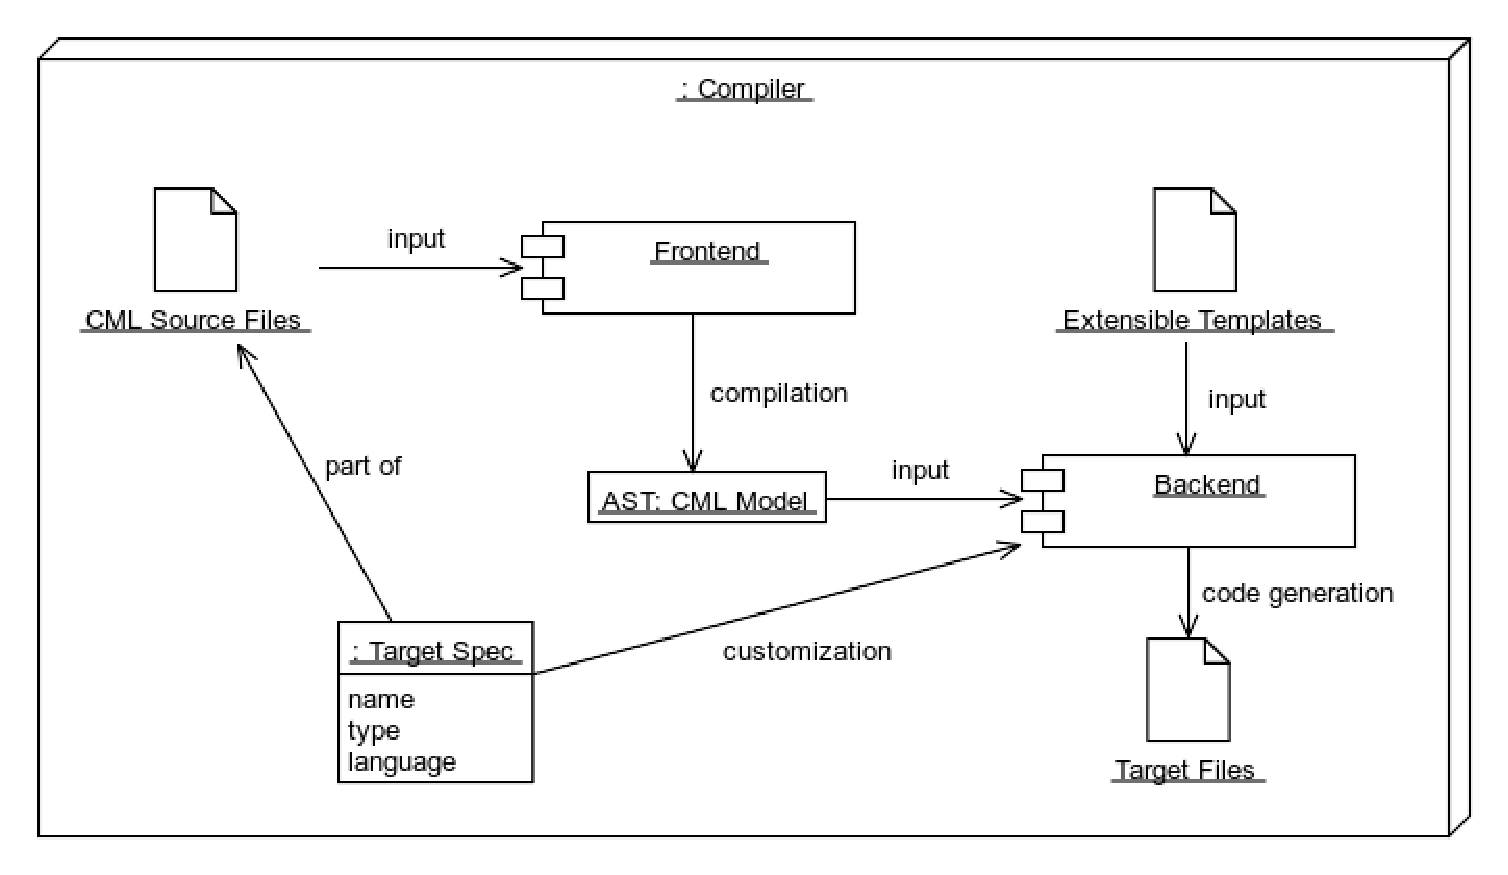
\includegraphics[width=\textwidth]{compiler/figure-overview}
\caption{An architectural overview of the CML compiler.}
\label{fig:overview}
\end{figure}

The CML compiler's overall architecture follows the standard compiler design literature \cite{torben}. An overview diagram of the architecture is shown in figure \ref{fig:overview}.
The two main components of the compiler,
and the artifacts they work with,
are presented in the next subsections.


\chapter{Concepts}
A \emph{concept} in the CML metamodel is used to represent anything
that has a coherent, cohesive meaning in a domain.
On the ER \cite{er} metamodel,
it corresponds to an \emph{entity};
on the UML \cite{uml} metamodel,
to a \emph{class}.
The CML \emph{concept} differs, however, from the UML \emph{class},
because it only contains \emph{properties},
while the UML \emph{class} may also have \emph{operations}.

Figure \ref{fig:ex:concepts} presents some examples of \emph{concepts} declared in CML.
As shown in the examples,
a \emph{concept} may have zero or more \emph{properties}
(\ref{sec:properties}),
and a \emph{property} may optionally declare a \emph{type}
(\ref{sec:primitive-types}, \ref{sec:collection-types}).
Also, as shown in the last example of figure \ref{fig:ex:concepts},
a \emph{concept} may specialize
(\ref{sec:generalization})
another \emph{concept}.

\begin{figure}
\verbatimfont{\small}
\begin{framed}
\verbatiminput{examples/concepts.cml}
\end{framed}
\caption{Concept Examples}
\label{fig:ex:concepts}
\end{figure}

Figure \ref{fig:stx:concept} specifies the syntax used
to declare a \emph{concept}.
The \textbf{concept} keyword is followed by a NAME.
Optionally, a list of other NAMEs may be enumerated,
referring to other \emph{concepts}
that are generalizations of the declared \emph{concept}.
Under the \textbf{concept} block,
a list of \emph{properties} may be declared as well.

\begin{figure}
\verbatimfont{\small}
\begin{framed}
\verbatiminput{grammar/Concepts.txt}
\end{framed}
\caption{Concept Declaration Syntax}
\label{fig:stx:concept}
\end{figure}


\section{Properties}
\label{sec:properties}
\begin{definition}
A \emph{property} in CML may hold values of primitive types,
in which case they correspond to \emph{attributes}
on the ER \cite{er} and UML \cite{uml} metamodels;
or they may hold references (or collections of references)
linking to instances of other \emph{concepts},
in which case they correspond to a \emph{relationship} on the ER metamodel,
and to \emph{associations} on the UML metamodel.
\end{definition}

\begin{examples}
Figure \ref{fig:ex:properties} presents some examples of \emph{properties} declared in CML.
As shown in the examples,
a \emph{property} may be an \emph{attribute} (\ref{ch:attributes})
of a \emph{primitive type} (\ref{sec:primitive-types}),
or represent the role/end of an \emph{association} (\ref{ch:associations}).
\end{examples}

\begin{figure}
\verbatimfont{\small}
\lstinputlisting[language=cml]{examples/properties.cml}
\caption{Property Examples}
\label{fig:ex:properties}
\end{figure}

\begin{concrete-syntax}
Figure \ref{fig:stx:property} specifies the syntax used
to declare a \emph{property}.
The NAME is followed by a \emph{typeDeclaration}
(\ref{sec:primitive-types} and \ref{sec:collection-types}).
Optionally, an \emph{expression} (\ref{ch:expressions}) may be specified
in order to set the initial value.
\end{concrete-syntax}

\begin{figure}
\verbatimfont{\small}
\lstinputlisting[language=antlr]{grammar/Properties.txt}
\caption{Property Declaration Syntax}
\label{fig:stx:property}
\end{figure}

\begin{abstract-syntax}
Figure \ref{fig:meta:property} presents the \emph{property} metamodel
in an EMOF \cite{mof} class diagram,
and figure \ref{fig:ast:property} specifies
the transformation
from the \emph{property} concrete syntax to its abstract syntax.
For each \emph{property} parsed by the compiler,
an instance of the \emph{Property} class will be created,
and its properties will be assigned
according to parsed information:

\begin{itemize}

\item \emph{name}:
assigned with the value of the terminal node NAME.

\item \emph{type}:
if \emph{typeDeclaration} is provided,
\emph{type} is set with the instance of the \emph{Type} class
matching the \emph{typeDeclaration}.

\item \emph{expression}:
if provided,
it contains the instance of the \emph{Expression} class
matching the parsed \emph{expression}.

\end{itemize}
\end{abstract-syntax}

\begin{figure}
\verbatimfont{\small}
\lstinputlisting[language=lsl]{ast/property.lsl}
\caption{Property AST Instantiation}
\label{fig:ast:property}
\end{figure}

\begin{constraints}
Figure \ref{fig:ocl:property} presents the invariants
of the \emph{Property} metaclass:

\begin{itemize}

\item \emph{unique\_property\_name}:
Each \emph{property} must have a unique NAME within its \emph{concept}
(\ref{ch:concepts}).

\item \emph{property\_type\_specified\_or\_inferred}:
Either the \emph{property} explicitly defines a \emph{type}
or it defines an \emph{expression},
from which the type is inferred.
That is required for both regular, slot-based \emph{properties}
(which may provide an \emph{initialization expression})
and \emph{derived properties}
(which may have an \emph{expression} defining the derivation).

\item \emph{property\_type\_matches\_expression\_type}:
When both a \emph{type} and \emph{expression} are provided by a \emph{property},
the \emph{type} inferred from the \emph{expression} should match
the declared \emph{type}.
That is required for both regular, slot-based \emph{properties}
(which may provide an \emph{initialization expression})
and \emph{derived properties}
(which may have an \emph{expression} defining the derivation).

\end{itemize}
\end{constraints}

\begin{figure}
\lstinputlisting[language=ocl_]{ocl/property.ocl}
\caption{Property Constraints}
\label{fig:ocl:property}
\end{figure}


\section{Generalization/Specialization}
\label{sec:generalization}
\begin{definition}
A \emph{concept} (\ref{ch:concepts}) in CML may be generalized by another \emph{concept}.
In other words, a \emph{concept} may be considered a specialization of another \emph{concept}.
Generalized \emph{concepts} have \emph{properties} (\ref{sec:properties})
that apply to a larger set of instances,
while specialized \emph{concepts} have \emph{properties}
that only apply to a subset of those instances.
In the UML \cite{uml} metamodel,
such generalization/specialization relationship between \emph{classes}
is known as \emph{generalization}, which is the name of the metaclass in the UML metamodel.
The original version of the ER \cite{er} metamodel lacked this kind of relationship
between \emph{entity types}.
\end{definition}

\begin{examples}
Figure \ref{fig:ex:generalization} presents some examples of
generalization/specialization relationships declared in CML.
As shown,
a \emph{concept} (\ref{ch:concepts}) may specialize zero or more other \emph{concepts}.
The latter are called the generalizations,
while the former is called the specialization.
A generalization, such as \textbf{Shape},
may define \emph{attributes} (\ref{ch:attributes}),
such as \textbf{color} and \textbf{area},
or also \emph{unidirecional associations} (\ref{sec:assoc-unidir}),
which are \emph{properties} (\ref{sec:properties}) shared among all its specializations.
Some of these \emph{properties} may be redefined by the some of the specializations,
as it is the case with the \emph{area} property,
which is redefined by \textbf{Rectangle}, \textbf{Rhombus} and \textbf{Square}.
Some specializations may also define new \emph{properties},
such as \textbf{width} and \textbf{height} in \textbf{Rectangle},
which characterize only instances of this specialization.
A \emph{concept} may be a specialization of two or more other \emph{concepts},
as seen with \textbf{Square},
which specializes both \textbf{Rectangle} and \textbf{Rhombus},
and thus can redefine \emph{properties} of both generalizations.
If a \emph{property} has been defined by more than one generalization,
then it must be redefined by the specialization
in order to resolve the definition conflict,
which is the case with \textbf{area} in \textbf{Square}. 
If a redefinition suitable for both generalizations is unattainable,
it may be an indication that either the specialization or the generalizations
are unsound from the domain's prospective.
\end{examples}

\begin{figure}
\verbatimfont{\small}
\lstinputlisting[language=cml]{examples/generalization.cml}
\caption{Generalization Examples}
\label{fig:ex:generalization}
\end{figure}

\begin{concrete-syntax}
Figure \ref{fig:stx:concept} specifies the syntax used
to declare a \emph{concept} (\ref{ch:concepts}),
and in turn its generalizations, if any.
A list of NAMEs may be enumerated after the declared \emph{concept}'s NAME,
referring to other \emph{concepts} that this concept is a specialization of.
\end{concrete-syntax}

\begin{abstract-syntax}
Figure \ref{fig:meta:concept} presents the \emph{concept} metamodel
in an EMOF \cite{mof} class diagram,
and figure \ref{fig:ast:concept} specifies
the \emph{concept} transformation
from its concrete syntax to its abstract syntax.
There is a unidirecional association in the \emph{Concept} class
that keeps track of the generalization/specialization relationships,
which is named \emph{generalizations}.
It is an \emph{ordered set} referencing all \emph{concepts}
whose NAMEs were enumerated in the \emph{GeneralizationList}
of the declared \emph{concept}.
\end{abstract-syntax}

\begin{constraints}
Figure \ref{fig:ocl:generalization} presents the invariants of the \emph{Concept} class
related to \emph{generalizations}:

\begin{itemize}

\item \emph{not\_own\_generalization}:
A \emph{concept} (\ref{ch:concepts}) may not be listed on its own \emph{GeneralizationList},
nor on the \emph{GeneralizationList} of its direct or indirect generalizations.

\end{itemize}
\end{constraints}

\begin{figure}
\lstinputlisting[language=ocl_]{ocl/generalization.ocl}
\caption{Generalization Constraints}
\label{fig:ocl:generalization}
\end{figure}


\section{Abstract Concepts}
\label{sec:abstract}

\chapter{Attributes}
\begin{definition}
In CML, \emph{attributes} are \emph{properties} (\ref{sec:properties})
of \emph{primitive types} (\ref{sec:primitive-types}).
They correspond to the \emph{Attribute} metaclass 
in the ER \cite{er} and UML \cite{uml} metamodels.
\emph{Attributes} serve as a \emph{slot} to hold a value of 
the specified \emph{primitive type}.
An initial value may be specified as an \emph{expression} (\ref{ch:expressions}).
An \emph{attribute}'s value may also be constantly
derived from an \emph{expression} (not only initially),
in which case it is called a \emph{derived attribute} (\ref{sec:derived-attributes}).
While initial values are only set when a \emph{concept} (\ref{ch:concepts})
is instantiated,
the value of \emph{derived attributes} are always evaluated 
from the given \emph{expression},
and they cannot be set any other way.
\end{definition}

\begin{examples}
Figure \ref{fig:ex:attributes} presents some examples of \emph{attributes} declared in CML.
As shown,
the attribute \textbf{a} is a regular attribute definition 
that specifies the \emph{primitive type} (\ref{sec:primitive-types})
of the values that can be held by the \emph{attribute}'s slot.
The attribute \textbf{b} is an example showing how an \emph{attribute}
can be defined with an initial value.
As shown by the attribute \textbf{c}, 
an attribute may be derived from an \emph{expression}
that refers to other \emph{attributes}.
In order to differentiate \emph{attributes} with initial values
from \emph{derived attributes},
a forward slash (``/'') prefixes the name of the latter.
Attributes \textbf{d} and \textbf{e} are examples
where the type of the attribute,
instead of being specified,
is inferred from the given \emph{expression}.
Type inference is possible for both regular, slot-based \emph{attributes}
and \emph{derived attributes} that provide an \emph{expression}.
\end{examples}

\begin{figure}
\verbatimfont{\small}
\lstinputlisting[language=cml]{examples/attributes.cml}
\caption{Examples of Attributes}
\label{fig:ex:attributes}
\end{figure}

\begin{concrete-syntax}
Figure \ref{fig:stx:property} specifies the syntax used
to declare any kind of \emph{property} (\ref{sec:properties}),
including \emph{attributes}.
The NAME of an \emph{attribute} is followed
by a \emph{typeDeclaration} of a \emph{primitive type}
(\ref{sec:primitive-types}).
Optionally, an \emph{expression} (\ref{ch:expressions}) may be specified
in order to set the initial value.
A \emph{derived attribute} must be prefixed with the forward-slash character,
as specified by DERIVED,
in which case the given \emph{expression} defines the value
of the \emph{attribute} at all times.
\end{concrete-syntax}


\chapter{Associations}
\begin{definition}
In CML,
an \emph{association} represents a relation between two \emph{concepts} (\ref{ch:concepts}),
where each \emph{concept} has an \emph{instance} in every tuple that is part of the relation.
When \emph{concepts} have an \emph{association},
its \emph{instances} are linked in such way that
it is possible to access an \emph{instance} of one \emph{concept}
from an \emph{instance} of the other \emph{concept}.
The UML \cite{uml} metamodel has a metaclass named \emph{Association} that has \emph{Property} instances,
whose \emph{types} are the \emph{Class} instances that are part of the \emph{association}.
In UML, the name of each \emph{Property} instance in the \emph{Association} metaclass
is known as the \emph{role} of the corresponding \emph{Class} in the \emph{association}.
On the CML metamodel, on other hand,
the \emph{Association} metaclass is only needed
when it is necessary to define \emph{bidirectional associations}.
For \emph{unidirectional associations},
only a \emph{property} is defined in the source \emph{concept},
making its \emph{type} the target \emph{concept}.
On the ER \cite{er} metamodel,
each \emph{association} is known as a \emph{relationship set},
and each tuple in this set is called a \emph{relationship}.
Unlike CML and UML,
the tuples in a \emph{relationship set} of an ER model
can be queried directly,
and no notion of \emph{property} is required as part of the \emph{entity type}
in order to access those \emph{relationships}.
As it is case for \emph{attributes} (\ref{ch:attributes}),
\emph{associations} in CML can also be derived from other \emph{associations}
(just as well as in UML);
they are called \emph{derived associations} (\ref{sec:derived-associations}).
\end{definition}

\begin{examples}
Figure \ref{fig:ex:associations} presents some examples of \emph{associations} declared in CML.
The concept \textbf{Vehicle} contains the property \textbf{driver},
which may optionally refer to an instance of \textbf{Employee},
meaning that a \textbf{driver} may or may not be assigned to a single \textbf{Vehicle}.
The concept \textbf{Vehicle} also has the property \textbf{owner},
which always refers to an instance of \textbf{Organization},
meaning that an \textbf{owner} must always be assigned to each instance of \textbf{Vehicle}. 
Similarly,
the concept \textbf{Employee} has the property \textbf{employer},
which must always be assigned to instance of \textbf{Organization}.
Just below the declaration of \textbf{Organization},
we observe an association named \textbf{Employment},
which enumerates two \emph{properties}:
the first is \textbf{employer} from the concept \textbf{Employee};
the second is \textbf{employees} from the concept \textbf{Organization}.
What this \emph{association} implies is a correspondence between these two properties.
Every time a reference to an instance of \textbf{Organization} is assigned to
the slot \textbf{employer} of an instance of \textbf{Employee},
a reference to this same instance of \textbf{Employee} must be assigned to
the slot \textbf{employees} of the \textbf{Organization} instance.
However,
since the \emph{type} of \textbf{employees}
in the concept \textbf{Organization}
is a sequence of \textbf{Employee} instances,
the reference to the instance of \textbf{Employee} will actually be added to the sequence,
along with the other instances already found in the sequence.
Thus, the association \textbf{Employment} actually characterizes a \emph{bidirectional association}.
The association \textbf{VehicleOwnership} is another example of a \emph{bidirectional association};
in this case,
between \textbf{Vehicle}'s \textbf{owner} property and \textbf{Organization}'s \textbf{fleet} property.
It can be noticed, though, 
in this second \emph{bidirectional association},
that the \emph{types} of the \emph{properties} are declared along with their names;
such a \emph{type} declaration,
in the \emph{association} declaration,
is optional in CML,
but must match the original \emph{property} declaration under the \emph{concept} declaration,
if present.
The \textbf{driver} property in the concept \textbf{Vehicle} is a different case,
since this \emph{property} does not participate in any \emph{association} declaration
in figure \ref{fig:ex:associations}.
That's because there is no corresponding \emph{property} in the concept \textbf{Employee}
representing the other end of the \emph{association}.
As such, the property \textbf{driver} is representing the source end of a \emph{unidirectional association}.
The property \textbf{drivers} in the concept \textbf{Organization} will be explained
in the section \ref{sec:derived-associations}.
\end{examples}

\begin{figure}
\verbatimfont{\small}
\lstinputlisting[language=cml]{examples/associations.cml}
\caption{Association Examples}
\label{fig:ex:associations}
\end{figure}


\chapter{Expressions}

\chapter{Targets}
\label{ch:targets}

\chapter{Modules and Libraries}

\appendix

\chapter{Concrete Syntax (Grammar)}
\clearpage
\section{ANTLR Grammar}

\begin{framed}
\verbatimfont{\small}
\begin{verbatim}
// Compilation Units:
\end{verbatim}
\verbatiminput{grammar/CompilationUnits.txt}
\begin{verbatim}
// Concept Declarations:
\end{verbatim}
\verbatiminput{grammar/Concepts.txt}
\begin{verbatim}
// Property Declarations:
\end{verbatim}
\verbatiminput{grammar/Properties.txt}
\begin{verbatim}
// Type Declarations:
\end{verbatim}
\verbatiminput{grammar/Types.txt}
\begin{verbatim}
// Target Declarations:
\end{verbatim}
\verbatiminput{grammar/Targets.txt}
\begin{verbatim}
// Names:
\end{verbatim}
\verbatiminput{grammar/Names.txt}
\begin{verbatim}
// Literals:
\end{verbatim}
\verbatiminput{grammar/Literals.txt}
\verbatiminput{grammar/Ignored.txt}
\end{framed}


\chapter{Abstract Syntax (Metamodel)}
\input{metamodel.tex}

\chapter{Abstract Syntax Tree (Instantiation)}
\input{ast.tex}

\backmatter

\bibliographystyle{plain}
\bibliography{references}

\end{document}
